\chapter{Background and Theory}
\label{ch:background}
The theoretical concepts of this thesis are overviewed in this chapter.
In an XFEL SPI experiment, single particles are illuminated by high-intensity coherent X-ray pulses
(\cref{fig:SPI_experiment}). 
We will describe how, on the basis of X-ray scattering theory, the structural information of molecules in SPI experiments is encoded\cite{lohReconstructionAlgorithmSingleparticle2009} in a sparse diffraction pattern--- Poisson sampled Ewald sphere slices of the
diffraction intensity with unknown orientations.

The XFEL SPI is an inverse problem of this encoding procedure and typically consists of
two steps in the data analysis pipeline: 
\begin{enumerate}
    \item diffraction intensity reconstruction: rebuild the three dimensional
        intensity distribution from sparse two dimensional diffraction patterns by assuming
        the diffraction intensity is continuous;
    \item phase retrieval: as the diffraction intensity only records the magnitudes information of
        the Fourier transform of the scattering factor with phase information missing recover
        the missing phase in the diffraction intensity by using prior information of the sample, such
        as size.
\end{enumerate}
In this thesis, we mainly focus on the data analysis and will provide needed theoretical and algorithmic
tools in the rest of this chapter.


\section{Basics of X-ray scalar diffraction theory}
\label{sec:scattering_diffraction}

In this section, we briefly describe the basics of X-ray diffraction to 
model the relation between structural information of single particles and 
their diffraction patterns recorded in experiment.

The interaction cross-section between photons and electrons essentially
consists of three parts when the energy of photons is in the range from
\SI{200}{eV} to \SI{500}{keV} \cite{raubenheimerLCLSIIStatusCW2015}:
\begin{enumerate}
    \item \emph{photoelectric effect}: core electrons are ejected by absorbing the
        energy of photons which cause vacancies. The photons are emitted 
        randomly when vacancies are filled another electrons;
    \item \emph{coherent scattering}: in this process, the total energy is conserved when photons
        are scattered by electrons. Those photons are coherent and their phases are decided by
        their relative position where they are scattered;
    \item \emph{Compton scattering}: this is an incoherent scattering process in which the incident photon transfers some of its energy to the electron.
\end{enumerate}

Taking the LCLS-II as an example\cite{raubenheimerLCLSIIStatusCW2015},
the photon energy range of SPI experiment with XFEL is around \SI{200}{eV} and
\SI{25}{keV}. In this range, the recorded photons are mainly from coherent
scattering\cite{hubbellReviewPhotonInteraction1999}. The fluorescence photons
(photoelectric effect) add an incoherent background to the diffraction patterns
and Compton photons are negligible. 

A classical model is adopted to illustrate the coherent scattered photons
encode particles' structures into their scattered angles and amplitudes.
When an electron (at the origin) is experiencing an oscillating incident plane electromagnetic wave, $\bvec E_\text{in}$,
it also emits electromagnetic radiation whose electric field part at the position $\bvec x$ could be expressed as
\begin{equation}
    \bvec{E}_\text{e}(\bvec x)=\frac{e^2}{4 \pi \varepsilon_{0} m_\text{e} c^{2}}
    \frac{\bvec{x} \times(\bvec{x} \times
    \bvec{E}_{\text{in}})}{|\bvec{x}|^{3}}\text{,}
    \label{eq:Esc}
\end{equation}
where $\varepsilon_{0}$ is the vacuum permittivity, $e$ and $m_\text{e}$ represent the charge and mass of electron respectively.
More often, the classical electron radius\cite{griffithsIntroductionQuantumMechanics2014}
\begin{equation}
    r_\text{e}=\frac{e^{2}}{4 \pi \varepsilon_{0} m_\text{e} c^{2}} \approx \SI{2.818e-15}{m}
    \label{eq:re}
\end{equation}
is introduced to simplify \cref{eq:Esc}. 
Multiple scattering of incident beam is ignored here since the specimen used in XFEP SPI experiment
is optical thin\cite{thibaultAlgorithmicMethodsDiffraction2007}.

In the XFEL SPI experiment (\cref{fig:lab_frame}), the distance between the illuminated particle and an observation point
on the detector, $R \sim \SI{1}{m}$, is several orders of magnitudes larger than
the scale of a nano-sized particle ($\sim\SI{10}{nm}$). Therefore, under the far field approximation\cite{jacksonClassicalElectrodynamics2007},
the electric field scattered by a particle with electron 
density $\rho(\bvec x_\text{p})$ at $\bvec x_\text{d}$ (usually the position of a detector pixel) 
is given by
\begin{equation}
    \bvec{E}(\bvec x_\text{d})=r_\text{e} \frac{\bvec x_\text{d} \times\left(\bvec x_\text{d}
    \times \bvec{E}_{\text{in}}\right)}{|\bvec x_\text{d}|^{3}}
    \int \rho(\bvec x_\text{p}) \exp\bigl[-2 \pi \img(\bvec k_\text{out} - \bvec k_\text{in})
    \cdot \bvec x_\text{p}\bigr] \dif \bvec x_\text{p} 
    \label{eq:Esc_int}
\end{equation}
where $\bvec k_\text{out}$ and $\bvec k_\text{in}$ are the scattered and incident wave vector, and
$(\bvec k_\text{out} - \bvec k_\text{in}) \cdot \bvec x_\text{p}$ is the difference between two
optical paths passing the origin and $\bvec x_\text{p}$.
Owing to the conservation of energy in elastic scattering, the wavelength of the scattered photon
is the same as the incident photon, or $\envert{\bvec k_\text{out}} = \envert{\bvec k_\text{in}}=
1/\lambda$, where $\lambda$ is the wavelength of X-ray, and the direction of $\bvec k_\text{out}$
is the same as the direction $\bvec x_\text{d}$. By introducing a new vector,
\begin{equation}
    \bvec k = \gls{torec}(\bvec x_\text{d}) = \bvec k_\text{out} - \bvec k_\text{in} = \envert{\bvec k_\text{in}}\hat{\bvec x}_\text{d} - \bvec k_\text{in}
    \label{eq:def_Krec}
\end{equation}
where $\hat{\bvec{a}}$ indicates the direction unit vector of a vector $\bvec{a}$,
and the Fourier transform of $\rho(\bvec x)$,
\begin{equation}
    \tilde{\rho}(\bvec k) = \Fourier[\rho](\bvec k)= \int \rho(\bvec x_\text{p}) \exp(- 2 \pi
    \img\bvec{k} \cdot \bvec x_\text{p}) \dif \bvec x_\text{p}\text{,}
    \label{eq:FT_rho}
\end{equation}
\cref{eq:Esc_int} could be rewritten as
\begin{equation}
    \bvec E(\bvec x_\text{d}) = \bvec E_\text{e} (\bvec x_\text{d})\cdot \tilde{\rho}\circ
    \torec(\bvec x_\text{d})\text{,}
    \label{eq:Esc_int2}
\end{equation}
where $E_\text{e}$ is defined in \cref{eq:Esc}.

%\Cref{eq:Esc_int} actual holds an assumption that electron density $\rho$ is independent on time.
%In other words, particle is frozen when it is illuminated by an XFEL pulse. 

%First, the thermal
%motion of particles could be neglected. For example, the weight $m$ and radius of gyration
%$r_\text{g}$ of lysozyme are \SI{14400}{\kilogram \per \kilo\mole} and
%\SI{15.20}{\angstrom}\cite{heNovelCorrelationProtein2003}.  In room temperature, the magnitude of
%thermal motion in \SI{1}{\femto\second}, including translation and rotation, is about
%\SI{1e-4}{\angstrom} by considering $3 k T / 2 = m v ^2/2 = m r_\text{g}^2 \omega^2 /2$, where $k$,
%$T$ are the Boltzmann constant and temperature, $v$ and $\omega$ are linear and angular speed. The
%angular speed is converted to linear speed by multiplying the radius of gyration. The value
%\SI{1e-4}{\angstrom} are much smaller than the radius of hydrogen atom (about
%\SI{1e-1}{\angstrom}). Second, the radiation damage on sample was studied with computer simulation
%in \cite{neutzePotentialBiomolecularImaging2000}.  Many facts are included: photoelectric, elastic
%and Compton scattering.  This study indicates that the damage could be outrun if pulse length is
%short enough.

The new vector, $\bvec k$, in \cref{eq:def_Krec} is a sphere centered at $\bvec k_\text{in}$ with
radius $1/\lambda$, which is known as \emph{Ewald sphere}.  The space of wave vectors is called
\emph{reciprocal space} (\cref{fig:lab_frame}), $\bbR_\text{rec}^3$ and the map between the laboratory frame
$\bbR_\text{lab}^3$ to the Ewald sphere in reciprocal space is denoted as $\torec$.

\begin{figure}[htpb]
    \centering
    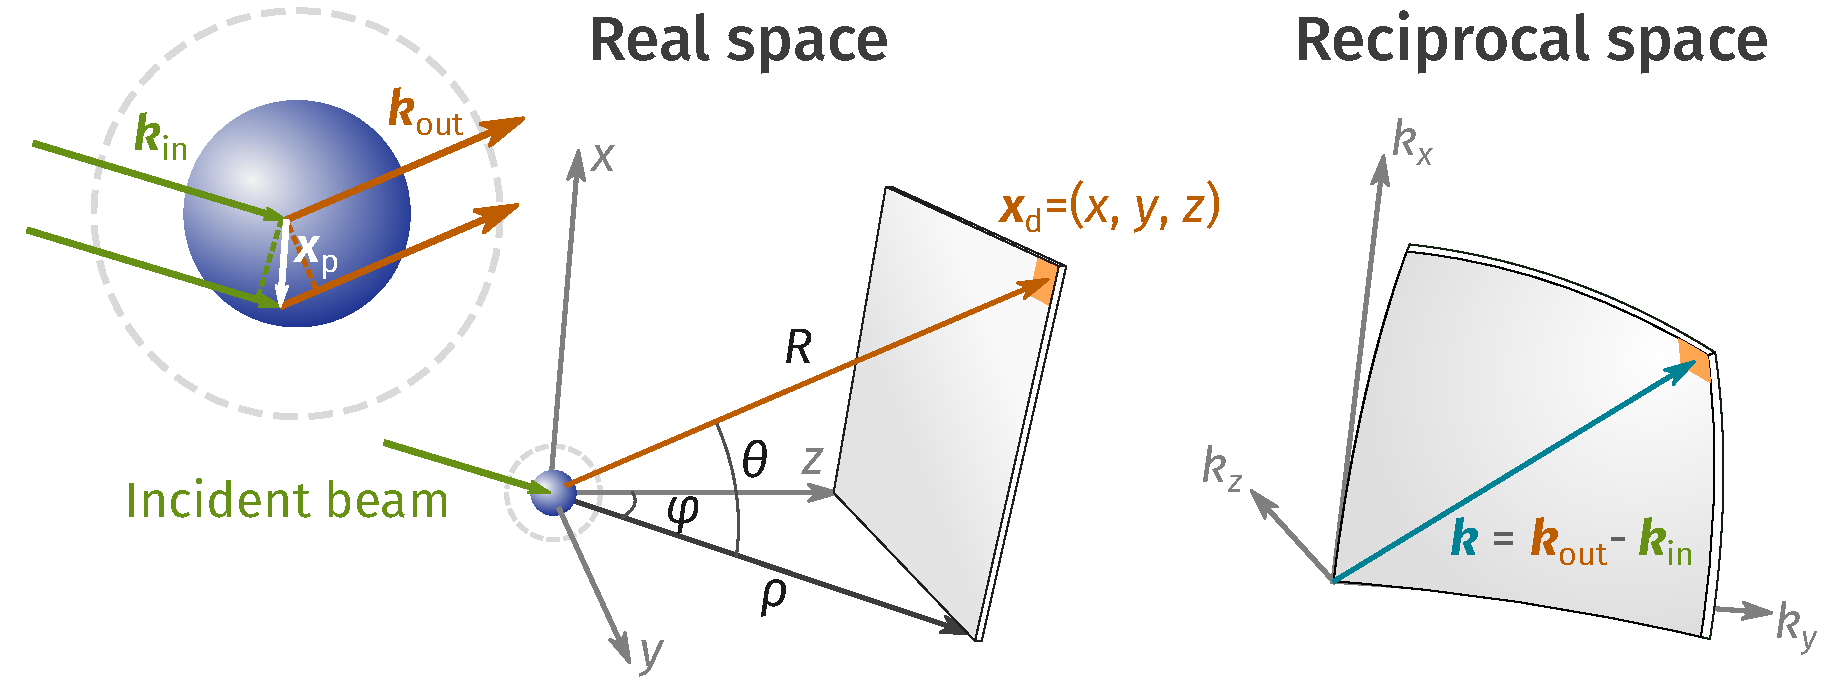
\includegraphics[width=0.96\textwidth]{pic/ill_lab.pdf}
    \caption[Lab coordinate system]{This figure illustrates the coordinate system of the real
        space (laboratory frame) and the reciprocal space and also shows the transformation between them.}
    \label{fig:lab_frame}
\end{figure}
